\section{Durchführung}
\label{sec:Durchführung}
Der Aufbau des Versuches entspricht in großen Teilen der schmatischen Skizze \ref{fig:skizze} für die Gegenfeldmemthode. In Abbildung
\ref{fig:aufbau} sind dann noch weitere notwendige Teile ergänzt, welche für die Durchführung benötigt werden. Dabei sind vor allem der 
Heizgenerator für das Einstellen der Temperatur nach Abschnitt \ref{sec:stör} und der XY-Schreiber für das Aufnehmen der Kurven von 
Bedeutung.
\begin{figure}[H]
    \centering
    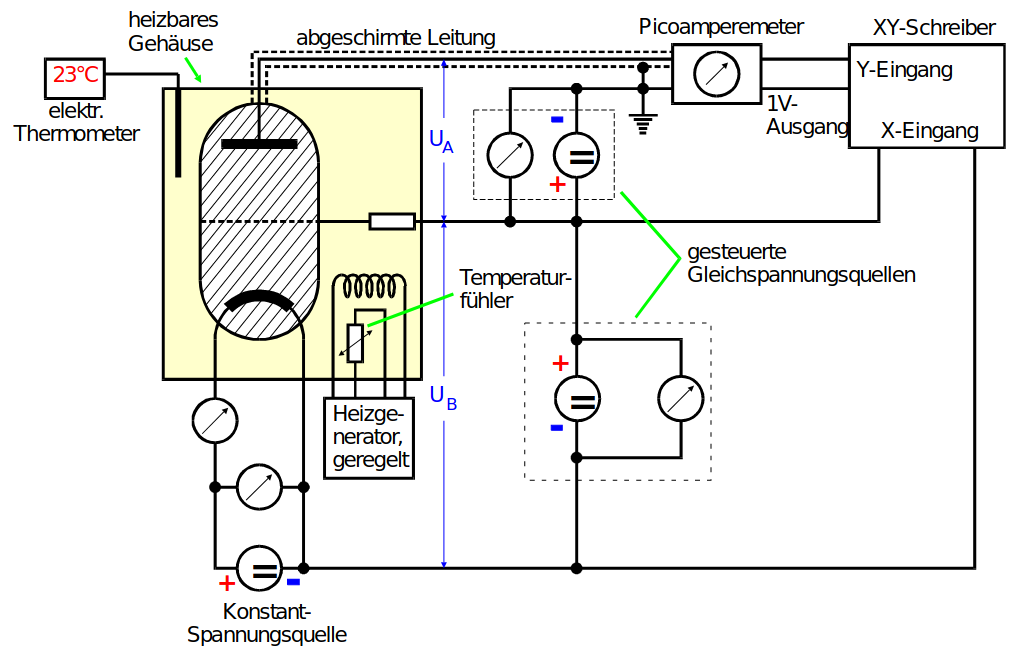
\includegraphics[scale = 0.5]{pictures/Aufbau2.png}
    \caption{Detaillierte Darstellung des Versuchaufbaus. \cite{AP01}}
    \label{fig:aufbau}
\end{figure}
\noindent
Vor jeder Messungen muss der XY-Schreiber so justiert werden, dass die aufgenommene Kurve möglichst auf DIN-A4 Größe skaliert ist. 
Dafür werden mit den auf dem Schreiber verbauten Reglern der Nullpunkt und die Skalierung so lange verschoben, bis die Kurve den Anforderungen
entspricht. Dann wird auf dem eingespannten DIN-A4 Blatt die Skalierung bestimmt, indem Punkte in $\SI{1}{\volt}$ Abständen auf der 
X-Achse markiert werden. Erst dann werden die Aufzeichnungen begonnen.

\subsubsection*{Energieverteilung der Elektronen}
Zuerst wird die Energieverteilung der Elektronen gemessen. Dazu wird der XY-Schreiber so angeschlossen, dass der Auffängerstrom $I_A$ in 
Abhänigkeit der Bremspannung $U_A$ gezeichnet wird. Die Beschleunigungsspannung $U_B$ ist dabei konstant $\SI{11}{\volt}$. Die Kurve
wird dann jeweils zwei Mal bei zwei unterschiedlichen Temperaturen ($T_1=\SI{24}{\celsius}$, 
$\SI{140}{\celsius} \leq T_2 \leq \SI{150}{\celsius}$) aufgenommen. Dabei wird die Messung im Bereich $\SI{0}{\volt} \leq U_A \leq 
\SI{10}{\volt}$ vorgenommen. 

\subsubsection*{Ionisationsenergie der Hg-Atome}
Für die Messung der Ionisationsenergie wird nun die Bremspannung $U_A$ konstant bei $\SI{-30}{\volt}$ gehalten. Die Beschleunigungsspannung
$U_B$ wird mit der X-Achse des XY-Schreibers verbunden, sodass der Auffängerstrom $I_A$ in Abhänigkeit von $U_B$ aufgenommen werden kann. 
Die Temperatur wird diesmal zwischen $\SI{100}{\celsius}$ und $\SI{110}{\celsius}$ eingestellt. Die Kurve wird dann in einem
Bereich von $\SI{0}{\volt} \leq U_B \leq \SI{60}{\volt}$ aufgenommen. 

\subsubsection*{Bestimmung der Franck-Hertz-Kurve}
Die Frack-Hertz-Kurve wird für zwei verschiedene Temperaturen im Bereich von $(\num{160}-\num{200})\si{\celsius}$ erfasst. Dazu wird die 
Beschleunigungsspannung mit der X-Achse und der Auffängerstrom mit der Y-Achse verbunden. Gemessen wird in einem Bereich von 
$\SI{0}{\volt} \leq U_B \leq \SI{60}{\volt}$, wobei für die Bremspannung $U_A=\SI{-1}{\volt}$ gilt.